%%%% MAIN TEX FILE FOR THESIS %%%%

\documentclass[12pt, a4paper, twoside]{article}


%%% GENERAL FORMATTING STUFF %%%
%%% not necessary when using xelatex to compile %%%
% \usepackage[utf8]{inputenc}	% UTF8 encoding
\usepackage[T1]{fontenc} % Enables proper hyphenation
\usepackage{scrextend} % Font size stuff
\usepackage{listing} % Source code formatting
\usepackage{layout} % Layouting options
\usepackage{pdfpages} % Enable including full pdf pages


%%% GENERAL LAYOUT %%%
\usepackage[onehalfspacing]{setspace}
% Uses the package 'geometry' to define the format of the page:
\usepackage[
    a4paper, % A4 paper
    left=2.50cm, right=2.50cm, top=2.50cm, bottom=2.50cm, % 2.5 cm margin to the sides
    bindingoffset=10mm, % 10 mm offset for binding
    includeheadfoot % Include header and footer
]{geometry}


%%% SPECIFY FONT %%%

% Set main font (serif font)
% \usepackage{fontspec}\setmainfont{Baskerville}
\usepackage{fontspec}\setmainfont{Adobe Garamond Pro}
% \usepackage{fontspec}\setmainfont{New Caledonia LT Std}

% Set secondary font (sans serif font)
% \setsansfont{Helvetica Neue}
% \setsansfont{Rockwell}
\setsansfont{Futura}

% Defines \code command to switch to monospaced font
\usepackage{seqsplit} % Split long words
\newcommand{\code}[1]{\texttt{\seqsplit{#1}}}


%%% SECTION HEADER FONT %%%
\usepackage{titlesec}
\usepackage{sectsty}
\setcounter{secnumdepth}{4} % Enables numbering for paragraphs
% Section: smallcaps, LARGE, sans serif
\sectionfont{\bfseries\LARGE\sffamily}
% Subsection header: bold, large, sans serif
\subsectionfont{\bfseries\large\sffamily}
% Subsubsection header: bold, normal, sans serif
\subsubsectionfont{\normalfont\large\sffamily}
% Paragraph header: bold, normal, sans serif -> For results and methods of manuscripts
% \topparagraph -> adds linebreak after header (results)
% \paragraph -> no linebreak after header (methods)
\makeatletter
\renewcommand{\paragraph}{\@startsection{paragraph}{5}{\z@}%
  {3.25ex \@plus1ex \@minus.2ex}%
  {-1em}%
  {\normalfont\normalsize\sffamily}}
\newcommand{\topparagraph}[1]{\paragraph{#1}\mbox{}\\}


%%% HEADER & FOOTER %%%
\usepackage{fancyhdr}
\fancyhf{}
% Height of the header
\setlength{\headheight}{15pt}
% Current section name in header
\fancyhead[LE,RO]{\textsc{\leftmark}}
% Pagenumber in footer
\fancyfoot[C]{\thepage}


%%% FIGURES %%%
\usepackage{graphicx} % Allows changing figure sizes
\usepackage{subfigure} % Allows subfigures in figures
\usepackage{float}
\usepackage{ccaption}
\usepackage{caption}
% \usepackage{fltpage} % Allows captions on next page
% Path for all graphics
\graphicspath{ {figures/} }
% Recognizes .pdf and .png automatically
\DeclareGraphicsExtensions{.pdf, .png, .jpg}
% Separator in Label. E.g. Figure 1 | Bladiblubb...
\DeclareCaptionLabelSeparator{line}{ | }
% Font: Helvetica, fontsize 8pt, linehight 12pt
\DeclareCaptionFont{helv}{\mdseries\fontsize{8}{12}\sffamily}
\captionsetup[figure]{font=helv, labelfont=bf, labelsep=line}


%%% TABLES %%%
\usepackage{booktabs} % Better lines in tables
\usepackage{longtable} % Linebreaks in tables
\usepackage{multirow} % Multirow tables
\usepackage{rotating} % Rotate table pages
\usepackage{arydshln} % Draw dashlines
\usepackage{csvsimple} % Include csvs
\usepackage{array}
\captionsetup[table]{font=helv, labelfont=bf, labelsep=line} % Table captions


%%%% OTHER STUFF %%%%
\usepackage{acronym} % Allows to use acronyms
\usepackage{adjustbox} % Draw boxes 
\usepackage{lipsum} % Lorem ipsum text
% \usepackage{authblk} % Author formatting 
% \usepackage{bbding} % Pretty symbols

\usepackage[hidelinks]{hyperref} % Enable hyperlinks ([hidelinks] to disable)


%%% MATH SPECS %%%
% Defines how equations are displayed
\renewcommand{\theequation}{Equation \arabic{equation}}


%%% SCIENCE %%%
\usepackage{dnaseq}	% Nucleotide sequences
\usepackage{texshade} % Aligned sequences 
\usepackage[version=4]{mhchem} % Chemical formulae
\usepackage{siunitx} % SI units
\usepackage{amsmath} % Prettier formulae
\usepackage{listings} % um Code zu setzen


%%% CITATION & BIBLIORGRAPHY STYLE %%%
\usepackage[
    % Management engine
    backend=bibtex,
    % Style: Author, Year. E.g. (R Sanchez 2213)
    style=authoryear-comp,
    citestyle=authoryear-comp,
    bibstyle=authoryear,
    % Sort Citations by year
    sortcites=true,
    sorting=nyt,
    % Max 10 names in bibliography
    maxbibnames=10,
    % Max 2 name in citation
    maxcitenames=2,
    uniquelist=false,
    uniquename=init,
    % Initials
    giveninits=true,
    % DOI, ISBN, URL & eprint not shown in bibliography
    doi=true,
    isbn=false,
    url=false,
    eprint=false
]{biblatex}

% Define command to start bibliography
\newcommand{\beginbibliography}{
    % Add to Table of Contents
    \addcontentsline{toc}{section}{Bibliography}
    \printbibliography
    \clearpage
}

% Path to file exported from mendeley
\addbibresource{bib/thesis.bib}


%%% SUPPLEMENT %%%
% Define command to start Supplement
\newcommand{\beginsupplement}{
    % Set conter of tables and figures to 0
    \setcounter{table}{0}
    \renewcommand{\thetable}{S\arabic{table}}
    \setcounter{figure}{0}
    \renewcommand{\thefigure}{S\arabic{figure}}
}

%%% CHAPTER %%%
% Define command to start new chapter
\newcommand{\newchapter}[1]{
    % Set conter of tables and figures to 0
    \setcounter{table}{0}
    \setcounter{figure}{0}
    % Reset S naming for supplement
    \renewcommand{\thefigure}{\arabic{figure}}
    \renewcommand{\thetable}{\arabic{table}}
    \input{#1}
    \clearpage
}

%%% BLANK PAGE %%%
% Define command to insert blank page
\newcommand{\blankpage}{
    \newpage
    \thispagestyle{empty}
    \
    \newpage
}



%%%% ACTUAL DOCUMENT %%%%

\begin{document}

\begin{titlepage}
\centering

{DISS.\ ETH NO.\ XXXXX}\\

\vspace{2cm}

{\bfseries\sffamily\LARGE
Exploring brain organoid development with multi-omics in single-cells
}

\vspace{2cm}

{\large A thesis submitted to attain the degree of}\\
{\sc \large Doctor of Sciences} {\large of} {\sc \large ETH Zürich}\\
{\large(Dr.\ sc. ETH Zürich)}\\


\vspace{1cm}

{\large presented by}\\

\vspace{0.3cm}

{\sc \large Jonas Simon Fleck}\\
{\large M.Sc. Ruprecht-Karls-Universität Heidelberg, Germany\\}

\vspace{1cm}

{\large 
born on 26. September 1991\\
citizen of Germany\\
}

\vspace{2cm}

{\large
accepted on the recommendation of\\
Prof.\ Dr.\ Barbara Treutlein, examiner\\
Prof.\ Dr.\ Randall J. Platt, co-examiner\\
Prof.\ Dr.\ Fabian J. Theis, co-examiner\\
}

\vspace{2cm}

{\large
2022
}
	
\end{titlepage}
\clearpage

\pagenumbering{roman}
\begin{center}
    \large\textsc{Abstract}
\end{center}
\markboth{Abstract}{}
\addcontentsline{toc}{section}{Abstract}

During human brain development, cells undergo remarkable fate transitions to give rise to a vast diversity of cell types. This process is tightly coordinated by a complex regulatory landscape that guides cells towards their terminal fate. It has long remained challenging to explore the molecular mechanisms that shape this landscape in humans. The convergence of two new technologies now offers fresh possibilities to study human brain development: \textit{In vitro} brain models grown from human stem cells and single-cell genomics. 

In this thesis, we use brain organoids to model cell fate acquisition during early human brain development and probe them using modern single-cell technologies. In the first part, we address the challenge of systematically characterizing organoid phenotypes. For this, we develop VoxHunt, a novel computational tool to assess the regional composition of brain organoids by mapping them to large reference atlases. In the second part, we illuminate the gene regulatory events shaping brain region diversification. We generate a single-cell transcriptome and chromatin accessibility atlas over a dense time course of early organoid development. We develop Pando, a flexible framework for inferring gene regulatory networks (GRNs) from multi-modal datasets and use it to infer a global GRN underlying human brain organoid development. We apply pooled genetic perturbations to assess transcription factor requirement for brain region diversification and show that the GLI3 is required for cortical fate establishment in humans. In the third part we were curious how brain development is altered in autism spectrum disorder (ASD) and performed a pooled genetic screen of ASD risk genes. We show that perturbations in many ASD genes lead to alterations of cell fate establishment and identify an ASD-specific sub-GRN. Specifically, we find that perturbation of ARID1B leads to aberrant fate transitions towards oligodendrocyte precursor cells. In the last part, we extend our previous multiomic atlas of early human brain development to shed light on epigenetic mechanisms. We profile three histone modifications and mRNA expression in single cells over an organoid developmental time course and identify epigenetic switches controlling cell fate bifurcations. Through perturbation of epigenetic modulators, we further show that epigenetic regulation is required to stabilize fate commitment during early organoid development. 

In summary, we here present new methods and insights to help illuminate the regulatory landscape underlying human brain development. We also provide valuable multi-omic reference atlases of brain organoid development and pioneer the application of perturbation screens in organoids to systematically interrogate gene regulation. Altogether, this thesis provides a framework for how human organoid systems and single-cell technologies can be leveraged to reconstruct human developmental biology.



\clearpage

\begin{center}
    \large\textsc{Acknowledgements}
\end{center}
\markboth{Acknowledgements}{}
\addcontentsline{toc}{section}{Acknowledgements}

This thesis would not have been possible without the supervision, support, kindness and love I received from so many people throughout the years. I will certainly not be able to name everyone, so I want to start off with a big \textit{thank you} to everyone who made the last years such a fun, exciting, educational and rewarding experience. 

First, my deepest gratitude belongs to Barbara, for giving me the opportunity to work on exciting topics with a bunch of amazing people. Your awe-inspiring compentence and admirable kindness made every discussion with you an uplifting and insightful experience. A huge thanks also goes to Gray, your vision and passion for science sparks enthusiasm and reignited my motivation many times. The two of you have assembled a team of excellent scientists and created a space buzzing with innovation. It was just a blast to work with every single one in the TreutCamp ensemble, thanks to all of you! Particularly I want to express my gratitude towards Fátima, Sophie and Fides, the shared first authors of the studies presented here. Quite literally none of this would have been possible without your know-how and talent. I'll be forever grateful for your (sometimes also emotional) support. Moreover, a great thanks to Zhisong for beeing a guiding light especially in the first years of my PhD. I learned quite a bit of new skills over the years and I feel like I owe a significant portion of this to your deep knowledge and experience. 

I want to thank our external collaborators and co-authors from Vienna, Prof. Jürgen Knoblich and Dr. Chong Li, who gave me the phenomenal chance to expand my horizon and work on such an exciting project. 

I also want to thank Prof. Fabian Theis and his group, for the invitation to Munich and many fruitful and enlightening discussions. 

Additionally, I want to thank Prof. Fabian Theis along with Prof. Randall Platt, who kindly agreed to participate in my thesis examination committee and Prof. Sai Reddy for chairing the defense. 

I want to thank the Boehringer Ingelheim Fonds for the financial support throughout my PhD and various educational seminars. I'm very grateful to be part of the rich and lively BIF community. 

I want to thank Dr. Georg Zeller, my master thesis supervisor, for his support even during my PhD and for lastingly shaping my view on science. 

Science really wouldn't be as fun without all the fascinating scientific discussions with incredibly smart people. I therefore want to thank everyone who I had the pleasure of exchanging interesting ideas with, including (but certainly not limited to) Christoph Harmel, Dr. Bastian Rieck, Dr. Tomás Gomes, Gilles Gut, Dr. Giovanna Brancati, Dr. Qianhui Yu, Dr. Matteo Togninally, Dr. Doris Popovic, Dr. Akanksha Jain and Dr. Philipp Wahle. 

This also feels like the right place to thank Dr. Makiko Seimiya, Dr. Malgorzata Santel and Dr. Ryoko Okamoto for keeping the lights on in the wetlab (even though I wasn't really there a lot). 

I am also deeply grateful for all friends who made the last years worthwile. First and foremost, I have to thank Simon, Benny and Chris for beeing the best and closest long-distance friends one could ever wish for. Thank you for everything! For prophecies, conspiracies, new holidays, nights, days and simply for existing. I want to thank  Christoph, for walks and talks and herbs. Also Lisi, Jamie, Jana, the Brits, the Cocktail Crew, all climbing and bouldering buddies and everyone else who made my time in Basel so enjoyable. Thanks also to Phil, Nico, Jana, Lasse, Tob, Jyoti, Lizzy, Jutta, Jannik, Pascal, and everyone else who is sadly not in Basel (but mostly in Berlin). 

I'm also incredibly thankful for Juliane, who stuck with me throughout the years. You enrich my life in so many ways and you in bring out the best in me. You are amazing, and I love you. 

Zu guter Letzt möchte ich meiner Familie danken: Meiner Mutter Karin, meinem Bruder Sammy, meinen Großeltern Gerda, Horst, Helga und Ernst, meinem Stiefvater Stephan und meinen Stiefgeschwistern Jonas, Karen, Philipp und Anna. Eure unerschütterliche Unterstützung und Fürsorge hat mich durch mein Leben getragen und mich zu der Person gemacht, die ich heute bin. Ich hab euch unglaublich lieb. 




\clearpage


\tableofcontents
\clearpage

\blankpage

\includepdf[fitpaper=true, pages=-]{pdfs/chapter_1.pdf}

\pagestyle{fancy} % Fancy header and footer
\pagenumbering{arabic} 	

\newchapter{chapters/introduction.tex}

\blankpage

\includepdf[fitpaper=true, pages=-]{pdfs/chapter_2.pdf}

\newchapter{chapters/voxhunt.tex}

\blankpage
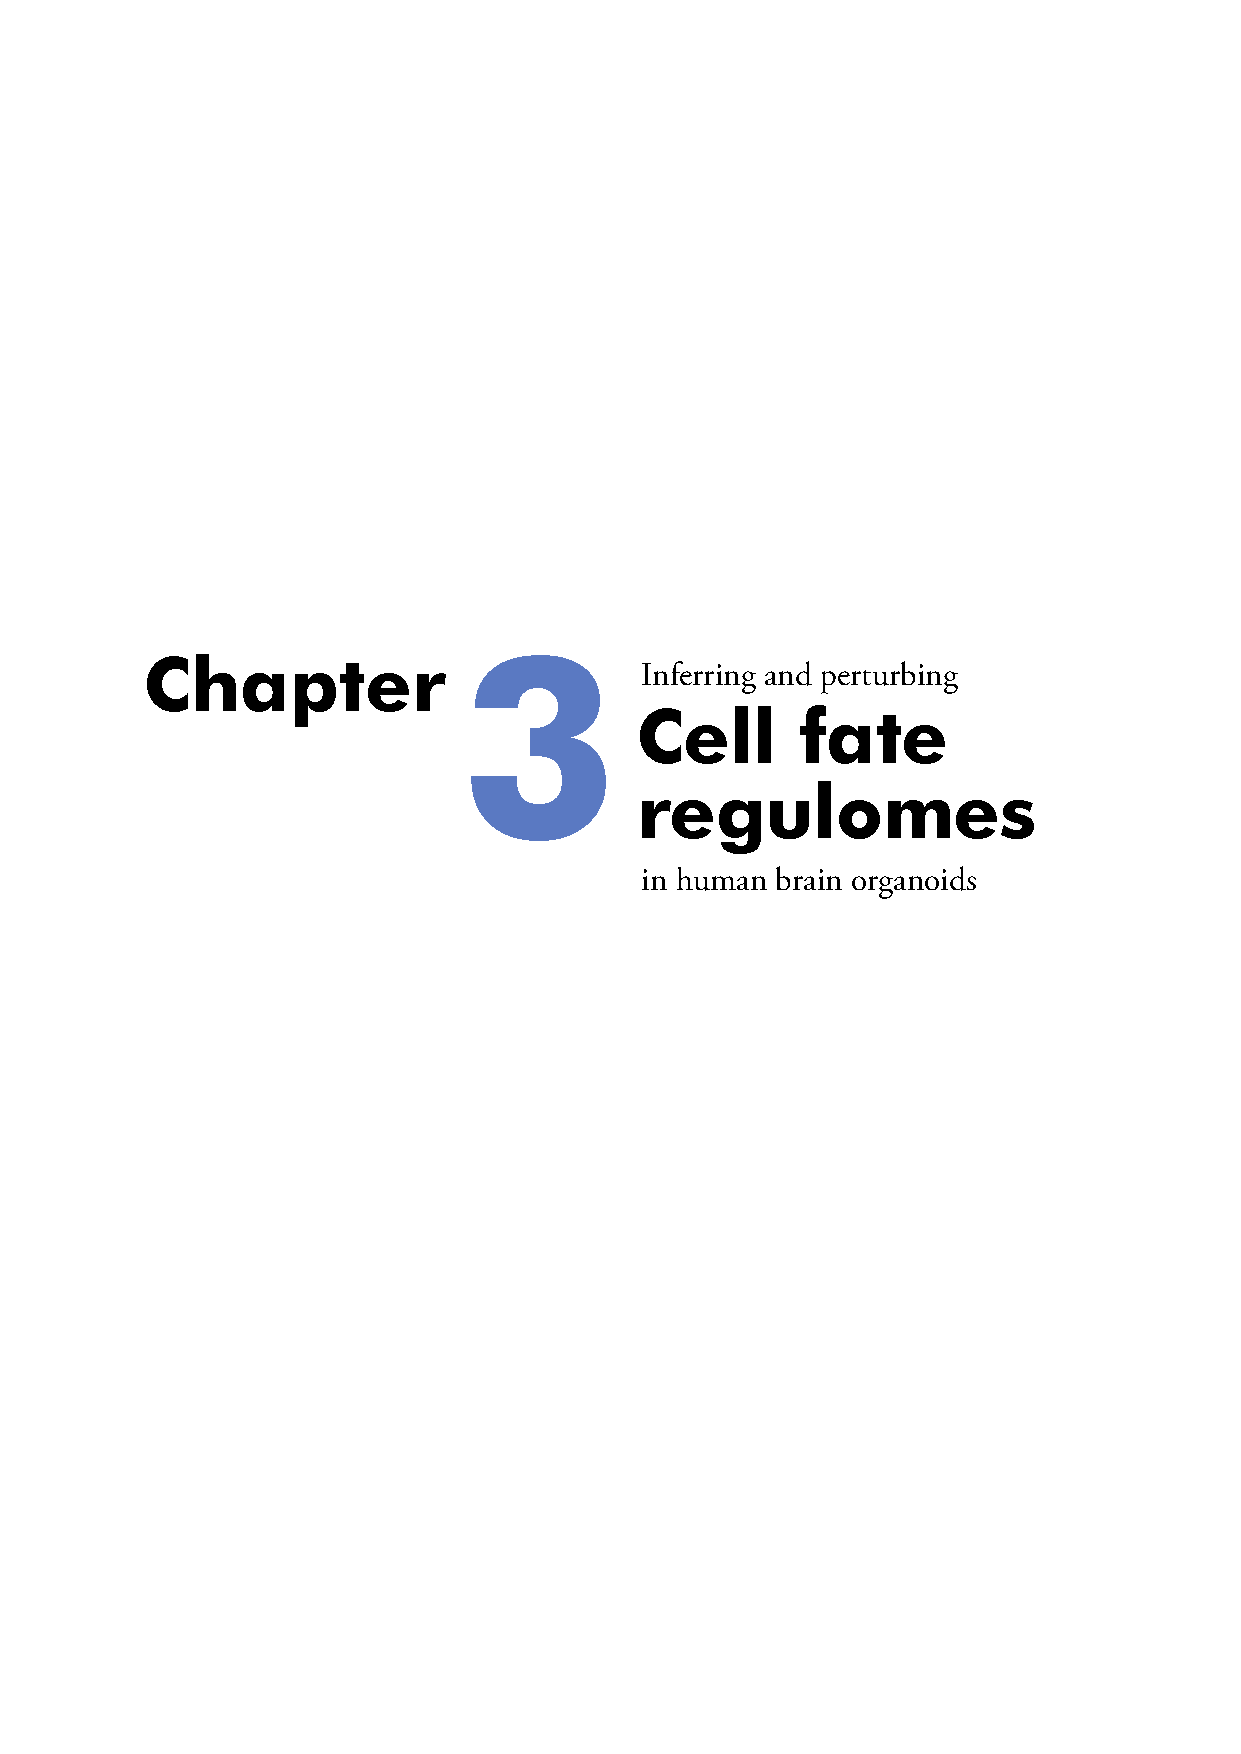
\includepdf[fitpaper=true, pages=-]{pdfs/chapter_3.pdf}

\newchapter{chapters/pando.tex}


\includepdf[fitpaper=true, pages=-]{pdfs/chapter_4.pdf}

\newchapter{chapters/asd.tex}

\blankpage

\includepdf[fitpaper=true, pages=-]{pdfs/chapter_5.pdf}

\newchapter{chapters/cnt.tex}

\blankpage

\includepdf[fitpaper=true, pages=-]{pdfs/chapter_6.pdf}

\newchapter{chapters/conclusions.tex}

\beginbibliography

\end{document}         


